\section{Results}
Analysis of differences in soil characteristics at landslide and non-landslide sites was conducted to evaluate the discriminative potential of the soil features used. This is important to understand whether the features carry enough information to support the machine learning classification process that follows. By comparing the data distribution of soil characteristics in both the landslide and no landslide groups, as illustrated in [\ref{fig:Violin-plot}], it can be observed that the two groups exhibit differences in distribution, although not always significant. Taking the \textit{S\_CLAY} feature as an example which represents the clay content in the subgrade it is evident that the no landslide group shows a data concentration between 20 and 40, with a median value tending to lie below 40. In contrast, the landslide group exhibits a concentration between 30 and 60, with a higher median than the no landslide group. This suggests that landslide-prone areas tend to have higher clay content compared to non-landslide areas.

To support this observation, a statistical analysis was conducted to calculate the \textit{p}-value using (\ref{eq:t_test}) or (\ref{eq:mann_whitney}) (the formula used depends on the data distribution, if the data distribution is normal then use t-test and u whitney-u otherwise). The \texttt{S\_CLAY} feature yielded a \textit{p}-value of $6.38 \times 10^{-5}$ (or 0.0000638), which is much smaller than the significance threshold of 0.05. This indicates a statistically significant difference between the two groups.

\begin{figure}[htbp]
    \centerline{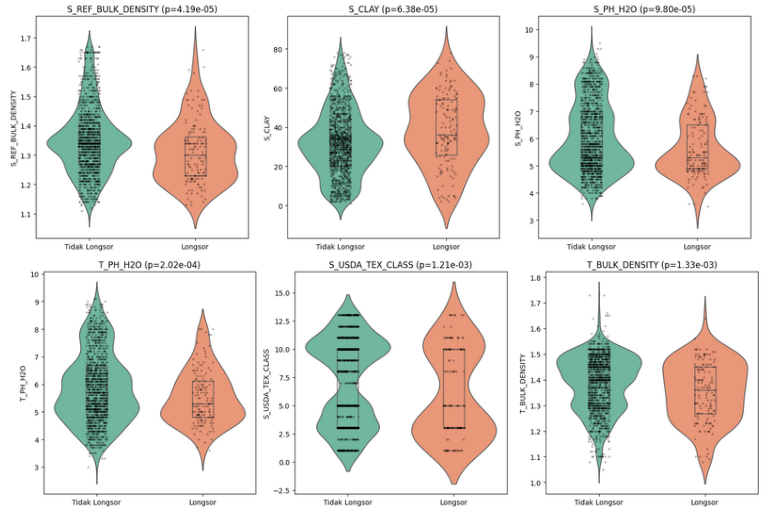
\includegraphics[width=\linewidth]{fig6.png}}
    \caption{Violin Plot of Topsoil vs Subsoil.}
    \label{fig:Violin-plot}
\end{figure}

After analyzing the differences in soil characteristics between landslide and non-landslide areas, the next step was to evaluate the predictive contribution of soil features at different depths. To this end, separate classification analyses were conducted using topsoil and subsoil features. The discriminative performance of these two feature sets was then evaluated using (ROC) curves and (AUC) values. The results, as shown in [\ref{fig:sub-top}], indicate that the model trained using the subsoil features achieved slightly superior predictive performance with an AUC value of 0.7205, compared to the model using the topsoil features with an AUC of 0.6984.

To further investigate the performance difference between the two soil layers, a feature importance analysis was conducted, as illustrated in [\ref{fig:feature-importance-top-sub}]. In the topsoil layer, the most influential features were primarily related to soil chemical properties, including Electrical Conductivity (T\_ECE), Calcium Carbonate (T\_CACO3), Total Exchangeable Bases (T\_TEB), and Organic Carbon (T\_OC). Meanwhile, in the subsoil layer, Calcium Carbonate (S\_CACO3) and Electrical Conductivity (S\_ECE) were the top contributors, followed by texture classification (S\_USDA\_TEX\_CLASS, United States Department of Agriculture Texture Classification) and Total Exchangeable Bases (S\_TEB). These findings highlight that subsoil characteristics particularly chemical and textural properties play a more critical role in predicting landslide susceptibility.

Collectively, these findings suggest that while both soil layers contribute valuable information, subsoil characteristics particularly those related to chemical composition and texture classification exhibit greater predictive power in landslide risk modeling compared to topsoil features.

\begin{figure}[htbp]
    \centerline{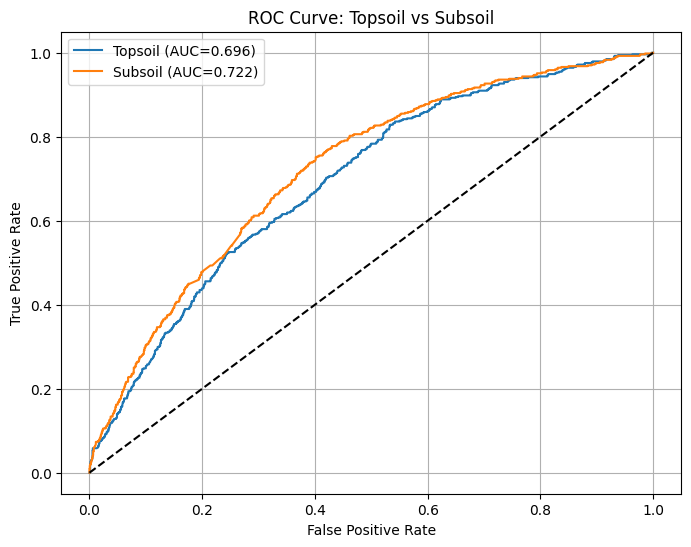
\includegraphics[width=\linewidth]{fig7.png}}
    \caption{ROC-AUC of Topsoil and Subsoil Layers.}
    \label{fig:sub-top}
\end{figure}
\begin{figure}[htbp]
    \centerline{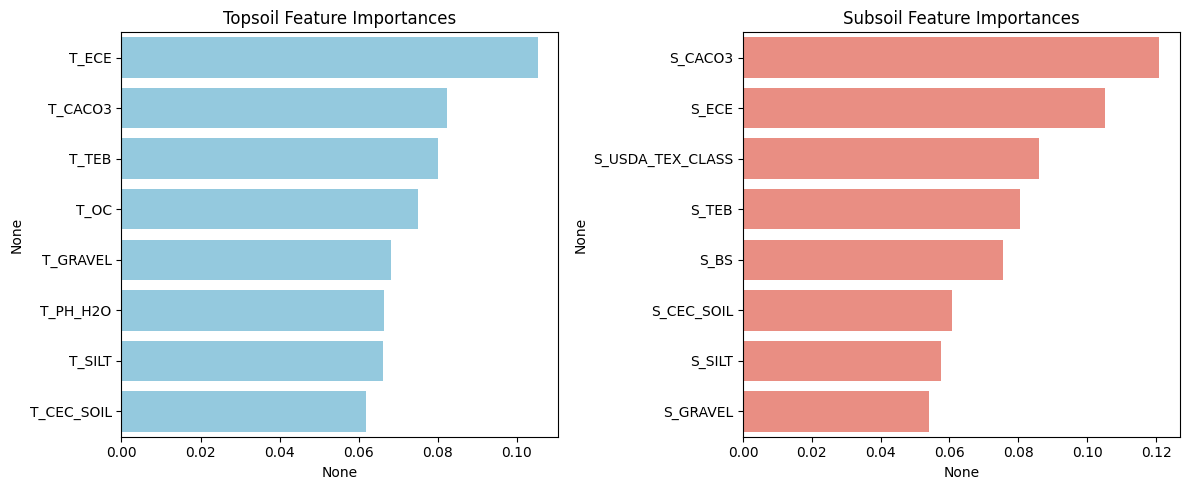
\includegraphics[width=\linewidth]{fig8.png}}
    \caption{Feature importance of Topsoil and Subsoil Layers.}
    \label{fig:feature-importance-top-sub}
\end{figure}

As a final step, a comprehensive model was trained by combining features from the topsoil and subsoil layers to evaluate their synergistic effects. The evaluation results of this combined model, visualized in the ROC curve in [\ref{fig:all-layers}], show a significant improvement in performance, achieving an AUC value of 0.85. This value far surpasses the performance of the model using only one of the layers separately.

This substantial improvement confirms that although the subsoil characteristics have a slightly more dominant predictive power, information from the topsoil also makes an essential complementary contribution. Thus, it can be concluded that holistic soil profile analysis---considering the interaction between both layers---is the most effective approach for landslide risk modeling with the highest accuracy.

\begin{figure}[htbp]
    \centerline{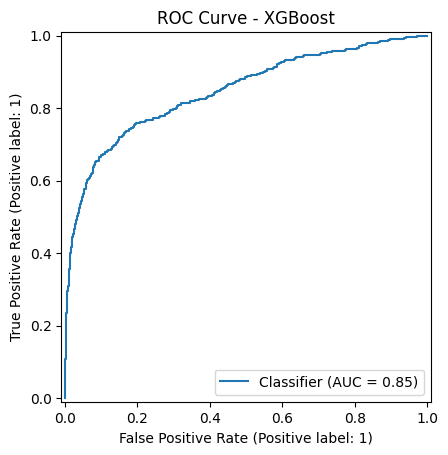
\includegraphics[width=\linewidth]{fig9.png}}
    \caption{ROC-AUC curve for all layers.}
    \label{fig:all-layers}
\end{figure}
\begin{figure}[htbp]
    \centerline{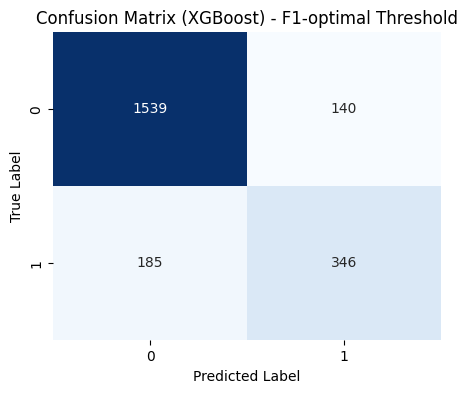
\includegraphics[width=\linewidth]{fig10.png}}
    \caption{Confusion matrix.}
    \label{fig:confusion-matrix}
\end{figure}

Figure~\ref{fig:confusion-matrix} shows that out of a total of 531 actual landslide events (class 1), the model correctly identified 346 of them (True Positive), while 185 events were missed (False Negative). For the non-landslide class (class 0), the model demonstrated strong performance with 1539 correct predictions (True Negative) and only 140 incorrect predictions (False Positive).

This is reflected in the classification report, where the model achieved a recall of 0.65 and a precision of 0.71 for the landslide class, resulting in an F1-score of 0.68. The overall accuracy of the model reached 85.29\%, indicating generally reliable predictive capability. With a weighted average F1-score of 0.85, the model demonstrates an effective balance between precision and recall across the dataset, validating the success of the optimization strategy on imbalanced data.
